\documentclass{article}
%packages
% \usepackage{tocloft}
\usepackage{polski}
\usepackage{amsmath}
\usepackage[utf8]{inputenc}
\usepackage{graphicx}
\usepackage{float}
\usepackage[font=small,labelfont=bf]{caption}
\usepackage[polish]{babel}
\usepackage{hyperref}
\hypersetup{
    colorlinks,
    citecolor=black,
    filecolor=black,
    linkcolor=black,
    urlcolor=black
}
% Variables
\newcommand{\HRule}{\rule{\linewidth}{0.5mm}}
\newcommand{\Prowadzacy}{dr hab. inż. Robert \textsc{Nowicki} prof. PCz}
\newcommand{\Ja}{Piotr \textsc{Filek}\\101311}
\newcommand{\Uczelnia}{ \textsc{\LARGE Politechnika Częstochowska}\\[1.5cm]}
\newcommand{\Przedmiot}{ \textsc{\Large Podstawy Sieci Komputerowych}\\[1.5cm]}
\newcommand{\TytulLaboratirum}{Laboratorium 1\\Sieci współdzielone}

%Equations list
% \newcommand{\listequationsname}{List of Equations}
% \newlistof{myequations}{equ}{\listequationsname}
% \newcommand{\myequations}[1]{%
% \addcontentsline{equ}{myequations}{\protect\numberline{\theequation}#1}\par}

\begin{document}
\begin{titlepage}
\begin{center}
\Uczelnia
% \textsc{\LARGE Politechnika Częstochowska}\\[1.5cm]
\Przedmiot% \textsc{\Large Final year project}\\[0.5cm]
\HRule\\[0.4cm]
{ \huge \bfseries \TytulLaboratirum \\[0.4cm] }
% { \huge \bfseries Large brewing techniques \\[0.4cm]}
\HRule\\[1.5cm]

% Author and supervisor
\begin{minipage}[t]{0.4\textwidth}
\begin{flushleft}\large
\emph{Autor:}\\
\Ja
\end{flushleft}
\end{minipage}
\begin{minipage}[t]{0.5\textwidth}
\begin{flushright} \large
\emph{Prowadzący:} \\
\Prowadzacy
\end{flushright}
\end{minipage}

\vfill

% Bottom of the page
{\large \DataLaboratorium}

\end{center}
\end{titlepage}
\begin{tableofcontents}
  \listoffigures
\end{tableofcontents}
\newpage
\section{Wstęp}

\begin{figure}[ht]
  \centering
  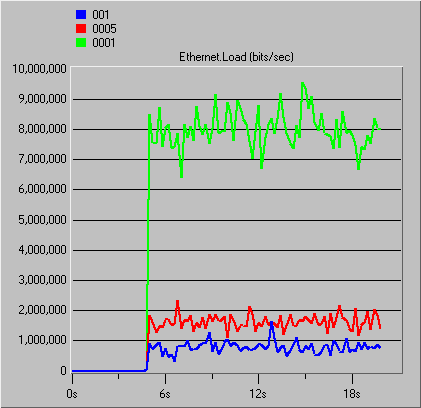
\includegraphics[width=0.8\textwidth]{screens/samo/load.png}
  \caption{test}
\end{figure}
\section{Przebieg zadań}
\subsection{Test 1}
\subsection{Test 2}

\begin{figure}[ht]
  \centering
  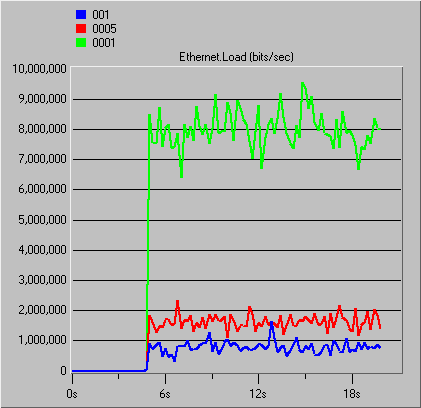
\includegraphics[width=0.8\textwidth]{screens/samo/load.png}
 \caption[Close up of \textit{Hemidactylus} sp.]
   {Close up of \textit{Hemidactylus} sp., which is
   part the genus of the gecko family. It is the
   second most speciose genus in the family.}
 \label{fig:example}
\end{figure}

\section{Wnioski}


Lubię placki

\end{document}